\documentclass[12pt,a4paper]{article}
\usepackage{graphicx}
\usepackage{fontspec}
\usepackage{geometry}
\geometry{left=1.25in,right=1.25in, top=1in,bottom=1in}
\setmainfont{Arial}
\usepackage{listings}
\title{24 Hour Project}
\author{Yuanyou Yao\\
and\\
Tianrun Wang}
\date{\today}
\begin{document}
\maketitle
\tableofcontents
\newpage
\section{Introduction}
The purpose of the article is to model the mortality associated with two pollution variables and three climate and socioeconomic variables. The data is collected from five Standard Metropolitan Statistical Areas (SMSA). We treat mortality, deaths per 100,000 popylation, as the response variable. NOX, SO2 associated with three climate and socioeconomic factors are the explanatory variables.\\
\newline
We decide to use \emph{Multi Linear Regression} to solve this problem. The problem states that two cities---Lancaster and York---have lower years of education because of their religion.Thus,we delete the data from Lancaster and York to make sure no other variables like religion will affect the analysis.   \\
\newline
After data cleaning, we run R to get two best fit{}ted models. To make the result more persuasive, we do other statistical tests to support our conclusions. Accordingly, all R codes are put in the appendix.
\newpage
\section{Methods and Models}
\subsection{Preparation}
We firstly delete Lancaster and York, and directly run a multiple linear regression and get the summary  which is listed below:
\newline
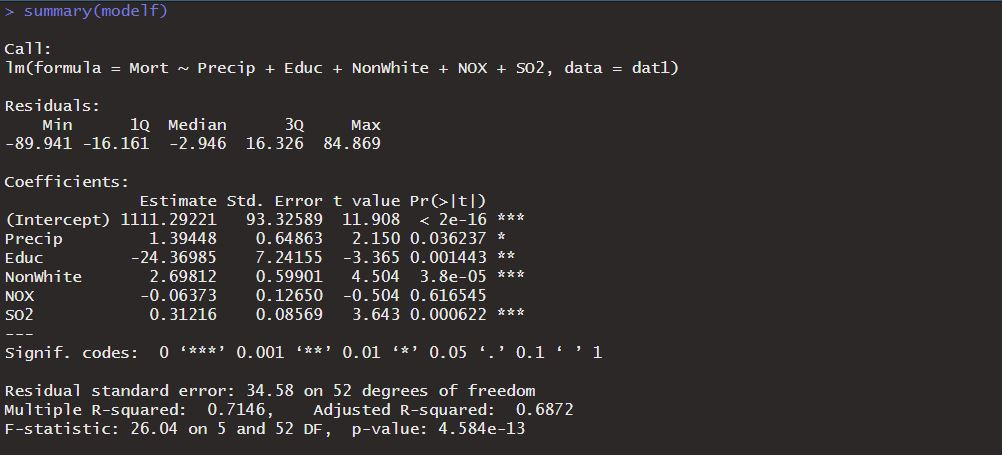
\includegraphics[scale=0.6]{all.JPG}
\newline
Then, we consider the multicollinearity. To diagnose, we perform Variance Inflation Factor(VIF), the result is listed below:
\newline
\begin{lstlisting}[language=R]
> vif(modelf)
  Precip     Educ NonWhite      NOX      SO2 
2.049842 1.573586 1.368329 1.688255 1.452572 
\end{lstlisting}
The largest VIF values of VIF$_K$ is considerably much smaller than 10, we can assert that multicollinearity problem does not affect inference. In addition, the correlation matrix support our assertion.
\begin{lstlisting}[language=R]
> cor(dat1[,c(-1,-2)])
             Precip Educ   NonWhite    NOX    SO2
Precip       1.00  -0.49    0.43      -0.48  -0.10
Educ        -0.49   1.00   -0.29       0.22  -0.27
NonWhite     0.43  -0.29    1.00       0.01   0.15
NOX         -0.48   0.22    0.01       1.00   0.41
SO2         -0.10  -0.27    0.15       0.41   1.00
\end{lstlisting}
\subsection{ANOVA}
We conduct an ANOVA table to see if the pollution variables have an effect on our response. \\
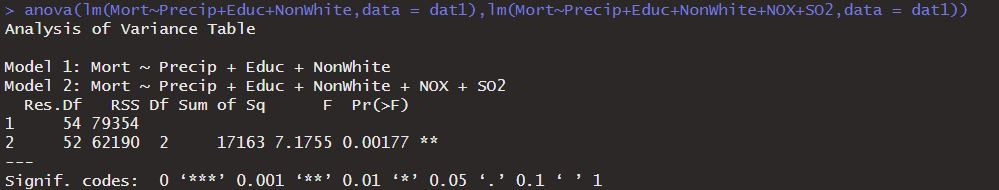
\includegraphics[scale=0.6]{ANOVA.JPG}
\newline
The result shows they are significant.
\subsection{All Possible Subsets Methods}
Because the number of variable is only 5, we can search all possible subset to choose the predictors. All possible subsets methods is performed and smallest BIC is the critrerion to pick the best model.\\
\newline
All the output is put into the appendix B. And we get our model:
\newline
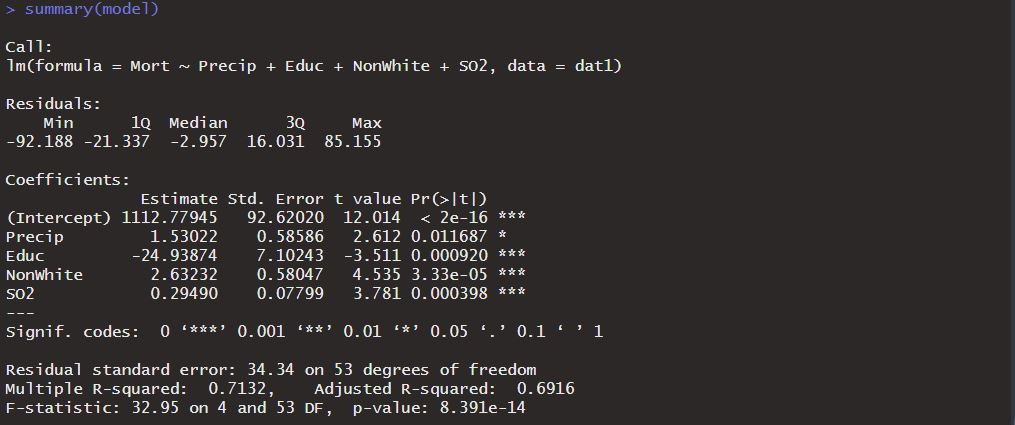
\includegraphics[scale=0.6]{b1.JPG}
\begin{center}
Mort $\sim$ Precip+Educ+NonWhite+SO2
\end{center}
With the coefficients:
\[
Mort=1112.77945+1.53022Precip-24.93874Educ+2.63232NonWhite+0.29490SO2
\]
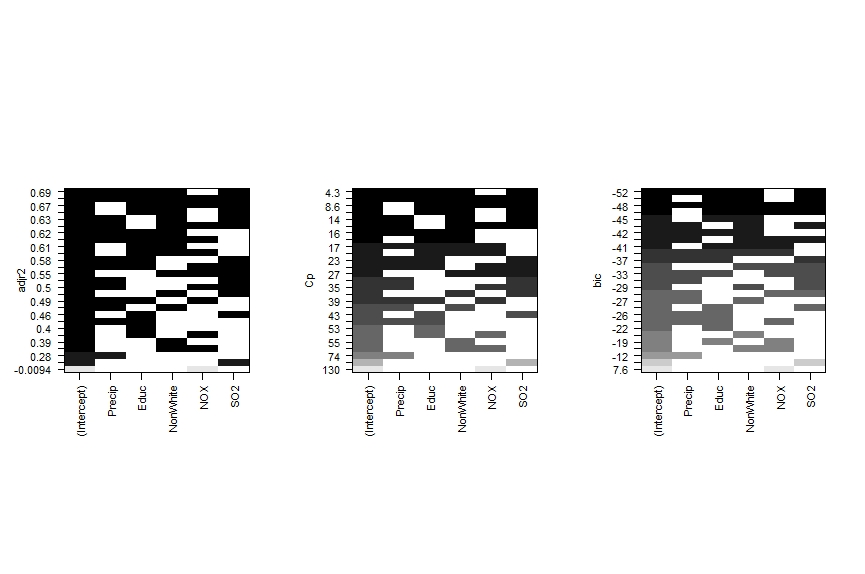
\includegraphics[scale=0.65]{apm.jpeg}
\newline
We get adjusted R$^2$=0.6916.\\
\newline
The image above shows the values of adjust $R^2$, C$_p$ Criterion and BIC when dif{}ferent variables are chosen. It satisfied the model we proposed before.
\subsection{Assumptions Check}
To use multi linear regression, we need to check several assumptions:
\begin{enumerate}
\item{Equal Variance}~{}
\newline
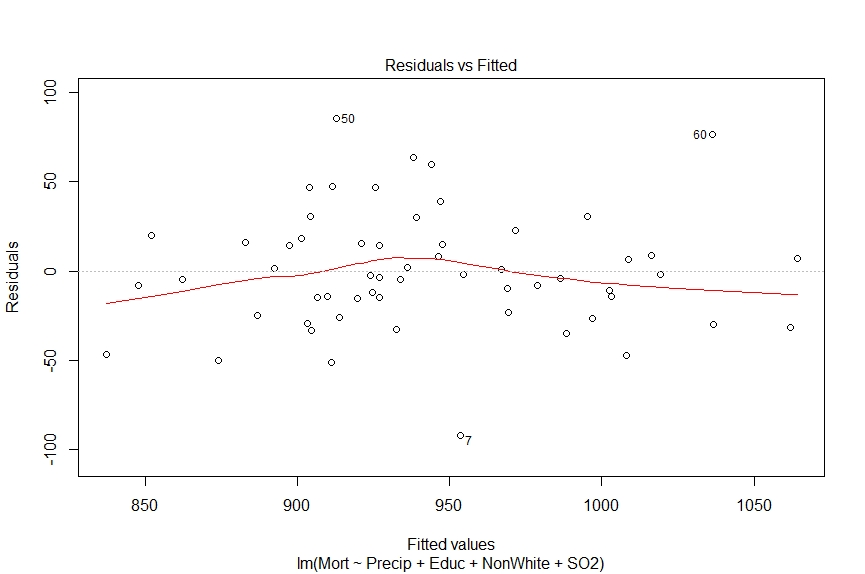
\includegraphics[scale=0.6]{ev.jpeg}
\newline
From the residuals vs fitted plot, we don't see the residuals getting larger or smaller. We may draw the conclusion that they are of equal variance.\\
\item{Normality}~{}
\newline
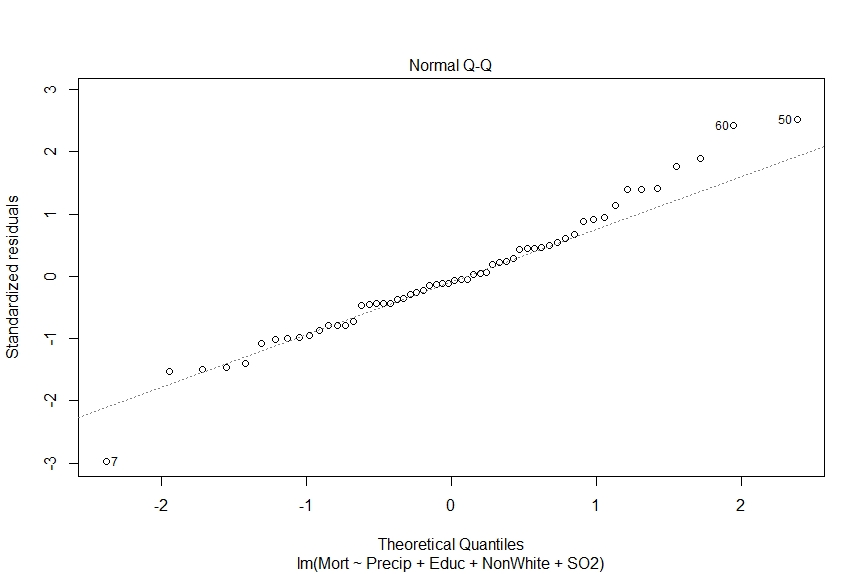
\includegraphics[scale=0.6]{qq.jpeg}
\newline
From the qq plot, we can see that normality assumption holds.\\
\item{Outliers}~{}
\newline
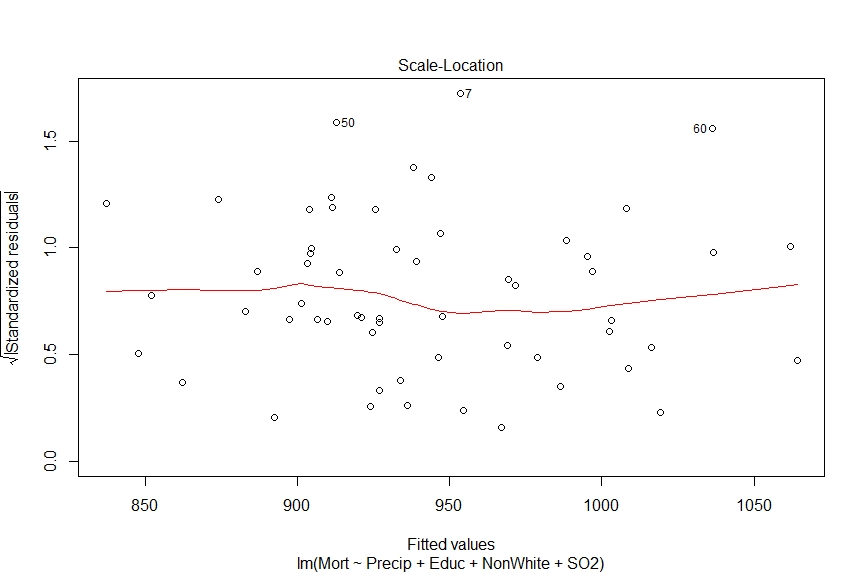
\includegraphics[scale=0.6]{3.jpeg}
\newline
We can see from the standardized residual plot that 7(Miami) is an outlier because of the rule of thumb that $\vert{r}\vert>3$\\
\newline
Also, we draw the studentized residual plot and see the same outlier.
\newline
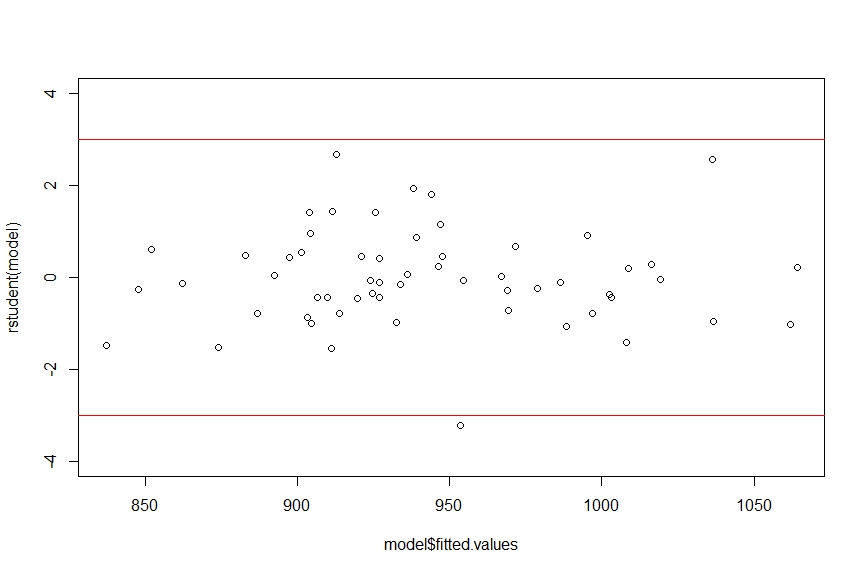
\includegraphics[scale=0.6]{rstu.jpeg}
\item{Strong Influence Point}~{}
\newline
We use the Cook's distance to identify Strong Influence Point.We use two rule of thumb $d>\frac{4}{n}$(the blue line) and $d>\frac{4}{n-p-2}$(the orange line). They all show 7(Miami) and 60(New orleans) are influential points. \\
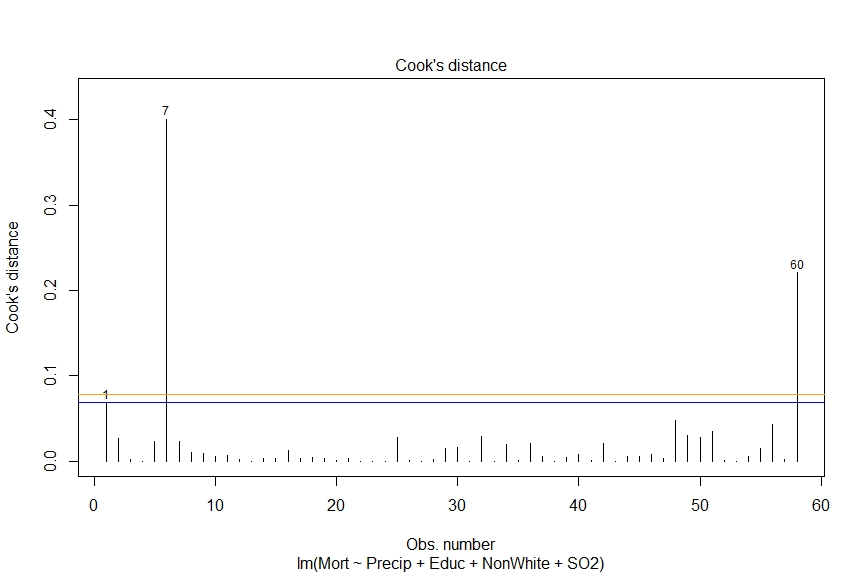
\includegraphics[scale=0.6]{cook.jpeg}
\end{enumerate}
\subsection{Remove the Outliers}
We remove the outliers and strong influence point(7 and 60) and refit the model. From the summary, we can see that the R square and Adjusted R square have increased(from 0.71 to 0.75, 0.69 to 0.73 seperately), which show our linear model working better.
\newline
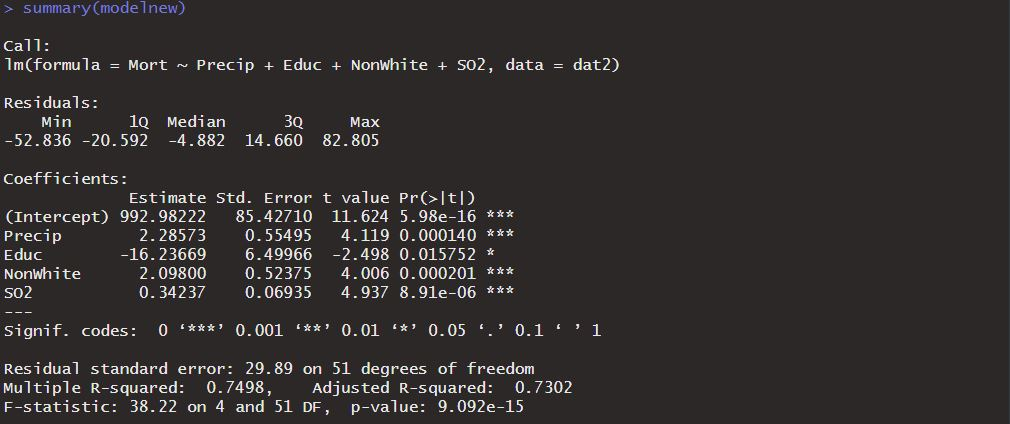
\includegraphics[scale=0.6]{Modelnew.JPG}
\subsection{Box-cox transformation}
We use the boxcox transformation to fit another model. We can calculate that when $\lambda=3.11$ the likelihood function gets its maximum.\\
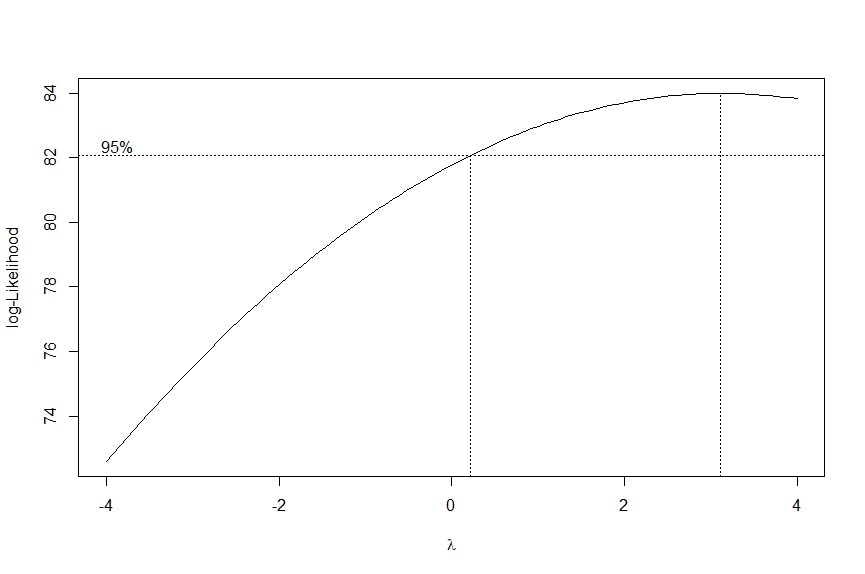
\includegraphics[scale=0.6]{boxcox.jpeg}
\newline
We choose $\lambda=3$ and fit this model:
\newline
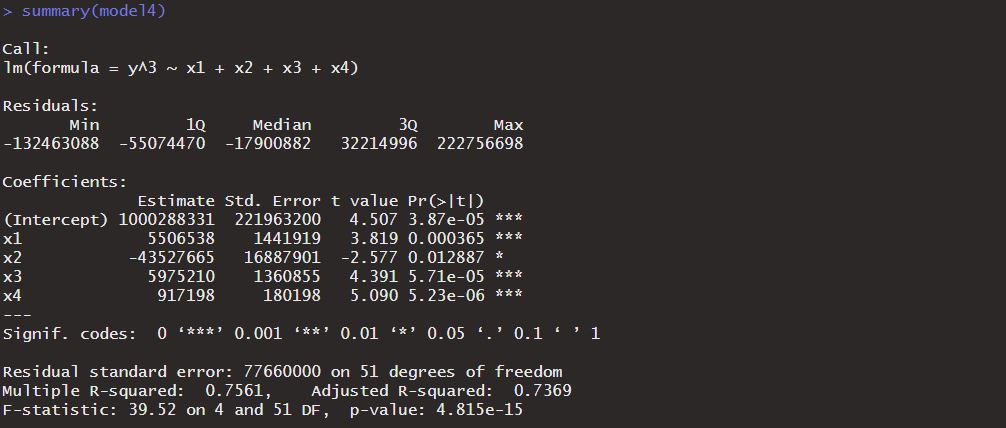
\includegraphics[scale=0.6]{BOXCOX.JPG}
\begin{center}
Mort$^3$ $\sim$ Precip+Educ+NonWhite+SO2\\
\end{center}
With the coefficients:\[Mort^3=1000288331+1000288331Precip-43527665Educ+5975210NonWhite+917198SO2\]

We get adjusted R$^2$=0.7369, showing the model works well.
\section{Results}
Two best fit{}ted models are\[Mort=1112.77945+1.53022Precip-24.93874Educ+2.63232NonWhite+0.29490SO2\] 
\begin{center}
and
\end{center}\[Mort^3=1000288331+1000288331Precip-43527665Educ+5975210NonWhite+917198SO2\]
\section{Limitations}
\begin{enumerate}
\item{}~{}
The model is too simple and cannot reflect the reality very well. 
\item{}~{}
The boxcox transformation doesn't produce a statisfying result.
\item{}~{}
While processing, we drop York and Lancaster at the beginning. If a proper method is used in our modeling without dropping these two observations, the result can be more accurate
\end{enumerate}
\section{Conclusions}
We firstly perform an ANOVA table to show that pollution variables are significant in our model. Secondly, we search through all possible subset to get the predictors. Then, we check the assumptions and delete the outliers and strong influential point. Lastly, we make a boxcox transformation to get another model.
\newpage
\appendix
\section{Appendix R Code}
\begin{lstlisting}
dat=read.csv("Data_24h_project.csv")
dat
#delete 4 and 20 line due to the question(Lancaster 
#and York)
dat1=dat[c(1:3,5:19,21:60), ]
modelf=lm(Mort~Precip+Educ+NonWhite+NOX+SO2
,data=dat1)
summary(modelf)
anova(lm(Mort~Precip+Educ+NonWhite,data = dat1),
lm(Mort~Precip+Educ+NonWhite+NOX+SO2,data = dat1))
#check for multicollinearity
require(car)
vif(modelf)
# result shows no ...

#model selection.
#due to there is only 5 varibles, we can get through
 #all subsets to find the best model

if (!require("leaps")) {
  install.packages("leaps")
  stopifnot(require("leaps"))
}

myleaps <- regsubsets(Mort~Precip+Educ+NonWhite+NOX+SO2
,data=dat1,nbest=8)
(myleaps.summary <- summary(myleaps)) # hard to interpret

# A better view:
bettertable <- cbind(myleaps.summary$which,
                     myleaps.summary$rsq, 
                     myleaps.summary$rss,
                     myleaps.summary$adjr2, 
                     myleaps.summary$cp, 
                     myleaps.summary$bic)
dimnames(bettertable)[[2]] <- c(dimnames(
myleaps.summary$which)[[2]],"rsq", "rss", "adjr2",
 "cp", "bic")
show(bettertable)
#we use the smallest BIC to pick the best model:Mort~
#Precip+Educ+NonWhite+SO2

par(mfrow=c(1,3), pty="s")
plot(myleaps, scale = "adjr2")
plot(myleaps, scale = "Cp")
plot(myleaps, scale = "bic")
#all shows the same result.

#outliers,normality,equal variance
model=lm(Mort~Precip+Educ+NonWhite+SO2,data = dat1)
summary(model)
par(mfrow=c(2,2))
plot(model,which = 1:4)

#the first plot shows equal variance.
#the second plot shows normality assumption holds
#the third plot shows an outlier 7(Miami)(because r>3)
# check studentized residuals
plot(model$fitted.values, rstudent(model))
plot(model$fitted.values, rstudent(model), ylim=c(-4,4))
abline(h=c(-3,3), col="red") # rule of thumb

p=5
n=58
plot(model, which = 4)
abline(h=qf(0.5, p, n-p), col="green")
abline(h=4/n, col="blue")
abline(h=4/(n-p-1-1), col="orange")
#7(Miami) and 60(New orleans) are influential points.

dat2=dat1[dat1$City!="Miami, FL" & dat1$City!=
"New Orleans, LA", ]
modelnew=lm(Mort~Precip+Educ+NonWhite+SO2,
data = dat2)
summary(modelnew)
summary(model)

library(MASS)
boxcox(modelnew,seq(-4,4,1/10))
y=dat2$Mort
x1=dat2$Precip
x2=dat2$Educ
x3=dat2$NonWhite
x4=dat2$SO2
bc=boxcox(y~x1+x2+x3+x4,lambda = seq(-4,4,1/10))
(lambda <- bc$x[which.max(bc$y)])

model4=lm(y^3~x1+x2+x3+x4)
summary(model4)

\end{lstlisting}
\section{Appendix Output of R}
\begin{lstlisting}
> myleaps <- regsubsets(Mort~Precip+Educ+NonWhite+
NOX+SO2, data=dat1,nbest=8)
>(myleaps.summary <- summary(myleaps)) # hard to interpret
Subset selection object
Call: regsubsets.formula(Mort ~ Precip + Educ + NonWhite + 
NOX + SO2, data = dat1, nbest = 8)
5 Variables  (and intercept)
         Forced in Forced out
Precip       FALSE      FALSE
Educ         FALSE      FALSE
NonWhite     FALSE      FALSE
NOX          FALSE      FALSE
SO2          FALSE      FALSE
8 subsets of each size up to 5
Selection Algorithm: exhaustive
         Precip Educ NonWhite NOX SO2
1  ( 1 ) " "    "*"  " "      " " " "
1  ( 2 ) " "    " "  "*"      " " " "
1  ( 3 ) "*"    " "  " "      " " " "
1  ( 4 ) " "    " "  " "      " " "*"
1  ( 5 ) " "    " "  " "      "*" " "
2  ( 1 ) " "    "*"  "*"      " " " "
2  ( 2 ) "*"    " "  " "      " " "*"
2  ( 3 ) " "    " "  "*"      " " "*"
2  ( 4 ) "*"    " "  "*"      " " " "
2  ( 5 ) " "    "*"  " "      " " "*"
2  ( 6 ) "*"    "*"  " "      " " " "
2  ( 7 ) " "    "*"  " "      "*" " "
2  ( 8 ) " "    " "  "*"      "*" " "
3  ( 1 ) " "    "*"  "*"      " " "*"
3  ( 2 ) "*"    " "  "*"      " " "*"
3  ( 3 ) "*"    "*"  "*"      " " " "
3  ( 4 ) " "    "*"  "*"      "*" " "
3  ( 5 ) "*"    "*"  " "      " " "*"
3  ( 6 ) " "    " "  "*"      "*" "*"
3  ( 7 ) "*"    " "  " "      "*" "*"
3  ( 8 ) "*"    "*"  " "      "*" " "
4  ( 1 ) "*"    "*"  "*"      " " "*"
4  ( 2 ) " "    "*"  "*"      "*" "*"
4  ( 3 ) "*"    " "  "*"      "*" "*"
4  ( 4 ) "*"    "*"  "*"      "*" " "
4  ( 5 ) "*"    "*"  " "      "*" "*"
5  ( 1 ) "*"    "*"  "*"      "*" "*" 
> # A better view:
>bettertable <- cbind(myleaps.summary$which,
                     myleaps.summary$rsq, 
                     myleaps.summary$rss,
                     myleaps.summary$adjr2, 
                     myleaps.summary$cp, 
                     myleaps.summary$bic)
>dimnames(bettertable)[[2]] <- c(dimnames(
myleaps.summary$which)[[2]],"rsq", "rss", "adjr2",
 "cp", "bic")
> show(bettertable)
  (Intercept) Precip Educ NonWhite         bic
1           1      0    1        0   0   0  -22.487738
1           1      0    0        1   0   0  -21.650853
1           1      1    0        0   0   0  -12.183221
1           1      0    0        0   0   1   -3.514529
1           1      0    0        0   1   0    7.634815
2           1      0    1        1   0   0  -44.662119
2           1      1    0        0   0   1  -31.707652
2           1      0    0        1   0   1  -29.425281
2           1      1    0        1   0   0  -26.760868
2           1      0    1        0   0   1  -25.706699
2           1      1    1        0   0   0  -25.539000
2           1      0    1        0   1   0  -18.670697
2           1      0    0        1   1   0  -18.500585
3           1      0    1        1   0   1  -49.180295
3           1      1    0        1   0   1  -44.072533
3           1      1    1        1   0   0  -42.349958
3           1      0    1        1   1   0  -40.628517
3           1      1    1        0   0   1  -37.186604
3           1      0    0        1   1   1  -33.739374
3           1      1    0        0   1   1  -27.648555
3           1      1    1        0   1   0  -25.402038
4           1      1    1        1   0   1  -52.142636
4           1      0    1        1   1   1  -47.486132
4           1      1    0        1   1   1  -40.996805
4           1      1    1        1   1   0  -39.242149
4           1      1    1        0   1   1  -33.318620
5           1      1    1        1   1   1  -48.364581
\end{lstlisting}
\end{document}
